\section{$\rho_1$ is not a 4-transposition}

\paragraph{}
By Lemma~\ref{min-4-trans}, at least one 4-transposition is needed. It can neither be at position $\rho_0$ by Lemma~\ref{exclude-0} nor in position $\rho_1$ by Theorem~\ref{exclude-1} therefore, $\rho_2$ must be the 4-transposition.

\paragraph{}
In the Theorem~\ref{find-2} we will use the method defined in~\ref{find-2} to find some sggis. In this case none of the generators of a sggi can be written as a product of the other. The permutation representation graph of those sggis are displayed in appendix~\ref{monodromy-5}. After that we will prove in Theorem~\ref{exclude-2} that none of those sggis satisfies the intersection property and thus none of them are string C-groups.

\begin{theorem}
  \label{find-2}
  The only permutation representation graph of rank 5 on 11 points are those displayed in appendix~\ref{monodromy-5} (p.~\pageref{monodromy-5}).
\end{theorem}

\begin{proof}
  In this case, we will start with the $\rho_2$ 4-transposition.

  \begin{figure}[H]
    \begin{center}
      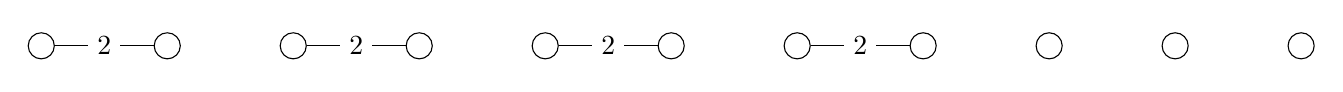
\begin{tikzpicture}[scale=.8]

        \begin{scope}[every node/.style={circle,draw}]
          \node (1)  at (-2,0)  {};
          \node (2)  at (0,0)  {};
          \node (3)  at (2,0)  {};
          \node (4)  at (4,0)  {};
          \node (5)  at (6,0)  {};
          \node (6)  at (8,0)  {};
          \node (7)  at (10,0)  {};
          \node (8)  at (12,0)  {};
          \node (9)  at (14,0)  {};
          \node (10)  at (16,0)  {};
          \node (11)  at (18,0)  {};
        \end{scope}

        \begin{scope}[every node/.style={fill=white}]

          \begin{scope}[every edge/.style={draw}]
            \path (1)  edge node {$2$} (2);
            \path (3)  edge node {$2$} (4);
            \path (5)  edge node {$2$} (6);
            \path (7)  edge node {$2$} (8);
          \end{scope}
        \end{scope}

      \end{tikzpicture}
      \caption{[1, 5, 1010, 232, 381]}
    \end{center}
  \end{figure}

\paragraph{}
The involutions $\rho_0$ and $\rho_4$ must commute with $\rho_2$ thus when adding their edges to the graph, only the pattern saw in~\ref{adding-patterns} are possible. But $\rho_0$ and $\rho_4$ must commute too. Thus they must form pattern saw in~\ref{todo}.

\paragraph{}
Since there is only one 4-transposition, there are only 12 edges available to link 11 points, 2 more than the minimum. Thus if a edge is added, it must link two distinct components, expect two times. Those two edges are called "joker" edges. When an alternating square is built, one of those edge is used, it is the same if a double edge is built.

\paragraph{}
A choice must be made among the three possibilities for each involution. We will prove that one involution must form an alternating square and that the other must make a double edge and link two fixed point of $\rho_2$.

\paragraph{}
First, we will prove that none of the involutions can make two double edge. Then we will prove that the same pattern cannot be used for both involutions.

\paragraph{}
Each pattern of Lemma~\ref{adding-patterns} use at least one edge. Thus none of the involution can choose to build two alternate squares because this pattern uses both "joker" edges and leaves nothing to the other involution which needs at least one.

\paragraph{}
The same choice cannot be made for $\rho_0$ and $\rho_4$. There is only three points fixed by $\rho_2$. If both involutions choose to make one alternating square and link two fixed points they must share at least one of the fixed points. Then there is two possibilities : only one vertex is share and there is a chain with an involution $\rho_0$ and $\rho_4$ but that is not a pattern of Proposition~\ref{todo} or they must form an alternating square. In this last case, there are three double edge: $(\rho_0, \rho_2), (\rho_2, \rho_4)$ and $(\rho_0, \rho_4)$. Thus three "joker" edges have been used but there are only two of them. The graph can never be connected\footnote{Add figure?}.

\paragraph{}
Otherwise if both involutions make an alternating square with $\rho_2$ there are two possibilities: the two squares can share some vertices or none.


\paragraph{}
If they share some vertices then a $\rho_0$ and a $\rho_4$ involution will share a vertex but that is forbidden by Lemma~\ref{0-4-no-share}.

\paragraph{}
If the two squares share no vertices the graph is the following.

\begin{figure}[H]
  \begin{center}
    \begin{tikzpicture}[scale=.8]

      \begin{scope}[every node/.style={circle,draw}]
        \node (1)  at (0,0)  {};
        \node (2)  at (0,2)  {};
        \node (3)  at (2,0)  {};
        \node (4)  at (2,2)  {};
        \node (5)  at (4,0)  {};
        \node (6)  at (6,0)  {};
        \node (7)  at (8,0)  {};
        \node (8)  at (10,0)  {};
        \node (9)  at (10,2)  {};
        \node (10)  at (12,0)  {};
        \node (11)  at (12,2)  {};
      \end{scope}

      \begin{scope}[every node/.style={fill=white}]

        \begin{scope}[every edge/.style={draw}]
          \path (1)  edge node {$0$} (3)
          \path (2)  edge node {$0$} (4);
          \path (1)  edge node {$2$} (2);
          \path (3)  edge node {$2$} (4);
          \path (8)  edge node {$2$} (9);
          \path (10) edge node {$2$} (11);
          \path (8)  edge node {$4$} (10);
          \path (9)  edge node {$4$} (11);
        \end{scope}
      \end{scope}

    \end{tikzpicture}
    \caption{[1, 5, 1010, 232, 381]}
  \end{center}
\end{figure}

\paragraph{}
All "joker" edges have been used so no more alternating square can be built. But the left square must be connected by a $\rho_1$ edge and the right one by a $\rho_3$ edge. We need to find a chain that connect the left square to the right square with only $\rho_1$ and $\rho_3$ edges. But that is impossible because the indices must be consecutive by Lemma~\ref{todo}.

\paragraph{}
Therefore one of the involution must build an alternating square and the other must build a double edge and link two fixed points. By duality, only the case where $\rho_4$ makes an alternating square will be considered and the other doubles an edge and links two fixed points.

\begin{figure}[H]
  \begin{center}
    \begin{tikzpicture}[scale=.8]

      \begin{scope}[every node/.style={circle,draw}]
        \node (1)  at (12,2)  {};
        \node (2)  at (12,0)  {};
        \node (3)  at (14,2)  {};
        \node (4)  at (14,0)  {};
        \node (5)  at (6,0)  {};
        \node (6)  at (4,0)  {};
        \node (7)  at (10,0)  {};
        \node (8)  at (8,0)  {};
        \node (9)  at (2,0)  {};
        \node (10) at (0,0)  {};
        \node (11) at (16,0) {};
      \end{scope}

      \begin{scope}[every node/.style={fill=white}]

        \begin{scope}[every edge/.style={draw}]
          \path (9)  edge node {$0$} (10);
          \path (7)  edge[bend right=30] node {$0$} (8);
          \path (1)  edge node {$2$} (2);
          \path (3)  edge node {$2$} (4);
          \path (5)  edge node {$2$} (6);
          \path (7)  edge[bend left=30] node {$2$} (8);
          \path (1)  edge node {$4$} (3);
          \path (2)  edge node {$4$} (4);
        \end{scope}
      \end{scope}

    \end{tikzpicture}
    \caption{The graph with only $\rho_0$ and $\rho_2$}
  \end{center}
\end{figure}

\paragraph{}
Now that all of our "joker" edges has been used, every other edge must link two different connected components of the graph.

\paragraph{}
Now the $\rho_3$ edge will be placed. It cannot be adjacent to the component consisting of the single $\rho_0$ edge or to the double edge. There are only three components that can be adjacent to such edge. Thus there are three places for two edges. The component that we are currently building must be linked to the rest of the graph by $\rho_1$ edges and a $\rho_1$ edge can only be connected to the single $\rho_2$ edge. This edge must so be connected by only one $\rho_3$ edge. The same applies for the fixed point that cannot be connected two times, otherwise two $\rho_3$ edges will share this vertex.

\paragraph{}
The square must thus be connected twice. There are three possibilities: the two connected vertices can be opposed or adjacent and, in this case, separated by a $\rho_1$ or a $\rho_3$ edge. This does not influence the position of the $\rho_1$ edges. It is possible to continue building the graph without having to deal with cases. Here is one of the possible graphs:

\begin{figure}[H]
  \begin{center}
    \begin{tikzpicture}[scale=.8]

      \begin{scope}[every node/.style={circle,draw}]
        \node (1)  at (0,2)  {};
        \node (2)  at (0,0)  {};
        \node (3)  at (-2,2)  {};
        \node (4)  at (-2,0)  {};
        \node (5)  at (-6,0)  {};
        \node (6)  at (-4,0)  {};
        \node (7)  at (-10,0)  {};
        \node (8)  at (-8,0)  {};
        \node (9)  at (-14,0)  {};
        \node (10) at (-12,0)  {};
        \node (11) at (2,0) {};
      \end{scope}

      \begin{scope}[every node/.style={fill=white}]

        \begin{scope}[every edge/.style={draw}]
          \path (9)  edge node {$0$} (10);
          \path (7)  edge[bend right=30] node {$0$} (8);
          \path (1)  edge node {$2$} (2);
          \path (3)  edge node {$2$} (4);
          \path (5)  edge node {$2$} (6);
          \path (7)  edge[bend left=30] node {$2$} (8);
          \path (2)  edge node {$3$} (11);
          \path (4)  edge node {$3$} (6);
          \path (1)  edge node {$4$} (3);
          \path (2)  edge node {$4$} (4);
        \end{scope}
      \end{scope}

    \end{tikzpicture}
    \caption{One of the graphs after placing $\rho_3$ edges}
  \end{center}
\end{figure}

\paragraph{}
Now the two edges of $\rho_1$ must be placed, the component containing the alternating square must be attached by its left end, the one that ends with a $\rho_2$ edge. The first two components must be linked together. The first component can be attached in two ways depending on the end choose to be attached. Here is one of the graphs:

\begin{figure}[H]
  \begin{center}
    \begin{tikzpicture}[scale=.8]

      \begin{scope}[every node/.style={circle,draw}]
        \node (1)  at (0,2)  {};
        \node (2)  at (0,0)  {};
        \node (3)  at (-2,2)  {};
        \node (4)  at (-2,0)  {};
        \node (5)  at (-6,0)  {};
        \node (6)  at (-4,0)  {};
        \node (7)  at (-10,0)  {};
        \node (8)  at (-8,0)  {};
        \node (9)  at (-14,0)  {};
        \node (10) at (-12,0)  {};
        \node (11) at (2,0) {};
      \end{scope}

      \begin{scope}[every node/.style={fill=white}]

        \begin{scope}[every edge/.style={draw}]
          \path (9)  edge node {$0$} (10);
          \path (7)  edge[bend left=30] node {$0$} (8);
          \path (5)  edge node {$1$} (8);
          \path (7)  edge node {$1$} (10);
          \path (1)  edge node {$2$} (2);
          \path (3)  edge node {$2$} (4);
          \path (5)  edge node {$2$} (6);
          \path (7)  edge[bend right=30] node {$2$} (8);
          \path (2)  edge node {$3$} (11);
          \path (4)  edge node {$3$} (6);
          \path (1)  edge node {$4$} (3);
          \path (2)  edge node {$4$} (4);
        \end{scope}
      \end{scope}

    \end{tikzpicture}
    \caption{One sggi on $A_{11}$ of rank 5}
  \end{center}
\end{figure}

\paragraph{}
There are 6 possible graphs but only one was built. The construction of the five remaining graphs is left to the reader. He can check that the graphs built match the graphs of appendix~\ref{monodromy-5}.

\end{proof}


\begin{theorem}
  \label{exclude-2}
  None of the groups represented by the graphs of appendix~\ref{monodromy-5} are C-groups.
\end{theorem}

\begin{proof}
  By the definition of a C-group, it is sufficient to find two subsets of generators $S_1$ and $S_2$ such that $\Gamma_{S_1} \cap \Gamma_{S_2} \neq \Gamma_{S_1 \cap S_2}$.

  \paragraph{}
  This proof is inspired by the section 4 of~\cite{leemansTransactions}.

  \paragraph{}
  In this case, they will be choose $S_1 = \{\rho_1, \rho_2\}$ and $S_2 = \{\rho_2, \rho_3, \rho_4\}$. Here $S_1 \cap S_2 = \{\rho_2\}$ and so $\Gamma_{S_1 \cap S_2} = \Gamma_{\rho_2}$ is a cyclic group of order 2. Hence, $\rho_2$ is an involution.

  \paragraph{}
  $S_1$ will be studied more deeply, only the $\rho_1$ and $\rho_2$ edges are kept in all the possible graphs. There are only two possible graphs:

  \begin{figure}[H]
    \begin{center}
      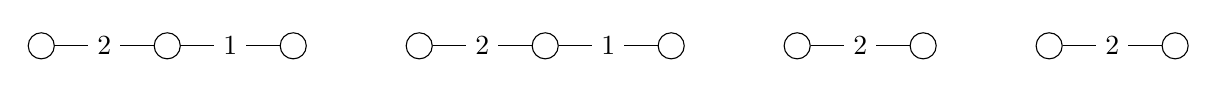
\begin{tikzpicture}[scale=.8]

        \begin{scope}[every node/.style={circle,draw}]
          \node (1)  at (-2,0)  {};
          \node (2)  at (0,0)  {};
          \node (3)  at (2,0)  {};
          \node (4)  at (8,0)  {};
          \node (5)  at (6,0)  {};
          \node (6)  at (4,0)  {};
          \node (7)  at (12,0)  {};
          \node (8)  at (10,0)  {};
          \node (9)  at (16,0)  {};
          \node (10) at (14,0)  {};
        \end{scope}

        \begin{scope}[every node/.style={fill=white}]

          \begin{scope}[every edge/.style={draw}]
            \path (2)  edge node {$1$} (3);
            \path (4)  edge node {$1$} (5);
            \path (1)  edge node {$2$} (2);
            \path (5)  edge node {$2$} (6);
            \path (7)  edge node {$2$} (8);
            \path (9)  edge node {$2$} (10);
          \end{scope}
        \end{scope}

      \end{tikzpicture}
      \caption{First possibility for $\Gamma_{S_1}$}
    \end{center}
  \end{figure}

  \begin{figure}[H]
    \begin{center}
      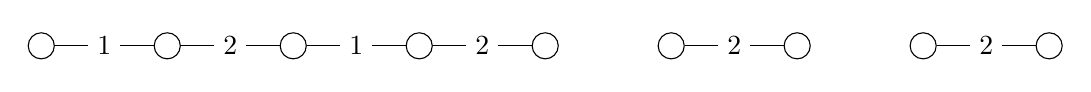
\begin{tikzpicture}[scale=.8]

        \begin{scope}[every node/.style={circle,draw}]
          \node (2)  at (0,0)  {};
          \node (3)  at (2,0)  {};
          \node (4)  at (4,0)  {};
          \node (5)  at (6,0)  {};
          \node (6)  at (8,0)  {};
          \node (7)  at (12,0)  {};
          \node (8)  at (10,0)  {};
          \node (9)  at (16,0)  {};
          \node (10) at (14,0)  {};
        \end{scope}

        \begin{scope}[every node/.style={fill=white}]

          \begin{scope}[every edge/.style={draw}]
            \path (2)  edge node {$1$} (3);
            \path (4)  edge node {$1$} (5);
            \path (3)  edge node {$2$} (4);
            \path (5)  edge node {$2$} (6);
            \path (7)  edge node {$2$} (8);
            \path (9)  edge node {$2$} (10);
          \end{scope}
        \end{scope}

      \end{tikzpicture}
      \caption{Second possibility for $\Gamma_{S_1}$}
    \end{center}
  \end{figure}

  \paragraph{}
  In the first graph, the permutation $(\rho_1 \rho_2)^2 \rho_1$ lets the points of the two isolated edges fixed because the permutation uses $\rho_2$ an even number of times. The points only linked by $\rho_1$ edges remain fixed too. But the point linked by $\rho_2$ edges in the big components are swapped. So it is possible to permute only two $\rho_2$ edges without touching the two others.

  \paragraph{}
  In the second graph, $(\rho_1\rho_2)^4 \rho_1$ gives the same result.

  \paragraph{}
  Now, let's study $S_2$, the disposition of the edges alongside the alternating square is very important. Therefore there are 3 possibilities:

  \begin{figure}[H]
    \begin{center}
      \begin{tikzpicture}[scale=.8]

        \begin{scope}[every node/.style={circle,draw}]
          \node (1)  at (-2,0)  {};
          \node (2)  at (0,0)  {};
          \node (5)  at (2,0)  {};
          \node (6)  at (4,0)  {};
          \node (7)  at (6,0)  {};
          \node (8)  at (6,2)  {};
          \node (9)  at (8,2)  {};
          \node (10) at (8,0)  {};
          \node (11) at (10,0) {};
        \end{scope}

        \begin{scope}[every node/.style={fill=white}]

          \begin{scope}[every edge/.style={draw}]
            \path (1)  edge node {$2$} (2);
            \path (5)  edge node {$2$} (6);
            \path (7)  edge node {$2$} (8);
            \path (9)  edge node {$2$} (10);
            \path (6)  edge node {$3$} (7);
            \path (10) edge node {$3$} (11);
            \path (7)  edge node {$4$} (10);
            \path (8)  edge node {$4$} (9);
          \end{scope}
        \end{scope}

      \end{tikzpicture}
      \caption{First possibility for $\Gamma_{S_2}$}
    \end{center}
  \end{figure}

  \begin{figure}[H]
    \begin{center}
      \begin{tikzpicture}[scale=.8]

        \begin{scope}[every node/.style={circle,draw}]
          \node (1)  at (-2,0)  {};
          \node (2)  at (0,0)  {};
          \node (5)  at (2,0)  {};
          \node (6)  at (4,0)  {};
          \node (7)  at (6,0)  {};
          \node (8)  at (6,2)  {};
          \node (9)  at (8,0)  {};
          \node (10) at (8,2)  {};
          \node (11) at (10,2) {};
        \end{scope}

        \begin{scope}[every node/.style={fill=white}]

          \begin{scope}[every edge/.style={draw}]
            \path (1)  edge node {$2$} (2);
            \path (5)  edge node {$2$} (6);
            \path (7)  edge node {$2$} (8);
            \path (9)  edge node {$2$} (10);
            \path (6)  edge node {$3$} (7);
            \path (10) edge node {$3$} (11);
            \path (7)  edge node {$4$} (9);
            \path (8)  edge node {$4$} (10);
          \end{scope}
        \end{scope}

      \end{tikzpicture}
      \caption{Second possibility for $\Gamma_{S_2}$}
    \end{center}
  \end{figure}

  \begin{figure}[H]
    \begin{center}
      \begin{tikzpicture}[scale=.8]

        \begin{scope}[every node/.style={circle,draw}]
          \node (1)  at (-2,0)  {};
          \node (2)  at (0,0)  {};
          \node (5)  at (2,0)  {};
          \node (6)  at (4,0)  {};
          \node (7)  at (8,2)  {};
          \node (8)  at (6,2)  {};
          \node (9)  at (6,0)  {};
          \node (10) at (8,0)  {};
          \node (11) at (10,0) {};
        \end{scope}

        \begin{scope}[every node/.style={fill=white}]

          \begin{scope}[every edge/.style={draw}]
            \path (1)  edge node {$2$} (2);
            \path (5)  edge node {$2$} (6);
            \path (7)  edge node {$2$} (8);
            \path (9)  edge node {$2$} (10);
            \path (6)  edge node {$3$} (9);
            \path (10) edge node {$3$} (11);
            \path (7)  edge node {$4$} (10);
            \path (8)  edge node {$4$} (9);
          \end{scope}
        \end{scope}

      \end{tikzpicture}
      \caption{Third possibility for $\Gamma_{S_2}$}
    \end{center}
  \end{figure}

  \paragraph{}
  The group generated by the right component is transitive because the component is connected. It's also 2-transitive, this can be checked by fixing the most right point and trying to move it's neighbor. For the first possibility this can be obtained by the permutation $\rho_2 \rho_4 \rho_3 \rho_2 \rho_3 \rho_2 \rho_3$. This can easily be proved for the three graphs and the proof is left to the reader.

  \paragraph{}
  The group is 2-transitive and thus primitive. The list of all primitive groups on seven points can be found in~\cite{buekenhout1996list}. The group is 2-transitive and so its order is a multiple of $7 \times 6 = 42$. But it is possible to find one subgroup by looking at the group generated by $\rho_2$ and $\rho_3$ only. This group is $D_{10}$ which is of order 10. The order of the group must also divide the order of those sub-groups.

  \paragraph{}
  Thus the order of the group must be a multiple of $7 \times 6 \times 5 = 210$. By looking at the list, there are only two primitive groups on seven points such that 210 divides they orders : $A_7$ and $S_7$. But the permutation $\rho_2$ is odd on those seven points, the only possibility is $S_7$.

  \paragraph{}
  But then every $\rho_2$ edge is an involution on those seven points. The other component, that only contains a $\rho_2$ edge must be there to keep the parity of the whole permutation. Therefore this group contains the same involution on four points that was found for $\Gamma_{S_1}$. This involution is in $\Gamma_{S_1}$ and in $\Gamma_{S_2}$ but not in $\Gamma_{\rho_2}$ thus $\Gamma$ does not satisfy the intersection property and is not a C-group.

\end{proof}

\paragraph{}
Now we have proven that there is no abstract polytopes of rank $5$ on $A_{11}$. Next we will prove the same for rank 4.
